\chapter{Подбор гиперпараметров и кросс-валидация}

\section{Решетчатый поиск гиперпараметров}

Для оптимизации силы и баланса штрафов применен поиск по сетке с 5-кратной кросс-валидацией (\texttt{GridSearchCV}):
\begin{itemize}
    \item Для \texttt{Lasso}: диапазон силы регуляризации $\alpha \in [10^{-4}, 10^{-3}, 10^{-2}, 0.1, 0.5, 1.0, 5.0, 10.0, 50.0, 100.0, 500.0, 1000.0]$;
    \item Для \texttt{ElasticNet}: комбинации силы $\alpha \in [10^{-4}, 10^{-3}, 10^{-2}, 0.05, 0.1, 0.5, 1.0, 10.0]$ и параметра соотношения $l_1\text{-ratio} \in [0.1, 0.3, 0.5, 0.7, 0.9, 0.95, 0.99]$.
\end{itemize}

Критерием оптимизации выбран коэффициент детерминации ($R^2$).

\begin{lstlisting}[language=Python]
from sklearn.model_selection import GridSearchCV, KFold

cv_kfold = KFold(n_splits=5, shuffle=True, random_state=42)

# Подбор гиперпараметра Lasso
grid_lasso = GridSearchCV(
    estimator=Lasso(random_state=42),
    param_grid={'alpha': [1e-4, 1e-3, 1e-2, 0.1, 0.5, 1.0, 5.0, 10.0, 50.0, 100.0, 500.0, 1000.0]},
    cv=cv_kfold, scoring='r2', n_jobs=-1
).fit(X_train_scaled, y_train)

# Подбор гиперпараметров ElasticNet
grid_elastic = GridSearchCV(
    estimator=ElasticNet(random_state=42),
    param_grid={'alpha': [1e-4, 1e-3, 1e-2, 0.05, 0.1, 0.5, 1.0, 10.0],
                'l1_ratio': [0.1, 0.3, 0.5, 0.7, 0.9, 0.95, 0.99]},
    cv=cv_kfold, scoring='r2', n_jobs=-1
).fit(X_train_scaled, y_train)
\end{lstlisting}

\section{Итоговая кросс-валидация и сводка результатов}

Для объективной проверки обобщающей способности выполнена 5-кратная кросс-валидация для пяти конфигураций моделей. Результаты представлены в таблице 4.

\begin{table}[H]
\centering
\small
\caption{Сводные результаты кросс-валидации и тестирования}
\resizebox{\textwidth}{!}{
\begin{tabular}{|l|c|c|c|c|}
\hline
\textbf{Модель} & \textbf{CV $R^2$ (mean $\pm$ std)} & \textbf{CV RMSE} & \textbf{Test RMSE} & \textbf{Test $R^2$} \\
\hline
LinearRegression & $0.8162 \pm 0.0151$ & 2.502 & 2.441 & 0.8242 \\
Lasso (базовый) & $0.8162 \pm 0.0151$ & 2.502 & 2.441 & 0.8242 \\
ElasticNet (базовый) & $0.6279 \pm 0.0155$ & 3.564 & 3.483 & 0.6380 \\
Lasso (оптимизированный) & $0.8162 \pm 0.0151$ & 2.502 & 2.441 & 0.8242 \\
ElasticNet (оптимизированный) & $0.8162 \pm 0.0151$ & 2.502 & 2.441 & 0.8242 \\
\hline
\end{tabular}
}
\end{table}

На рисунке 3 приведено наглядное сопоставление точности моделей на тестовой выборке до и после подбора гиперпараметров.

\begin{figure}[H]
    \centering
    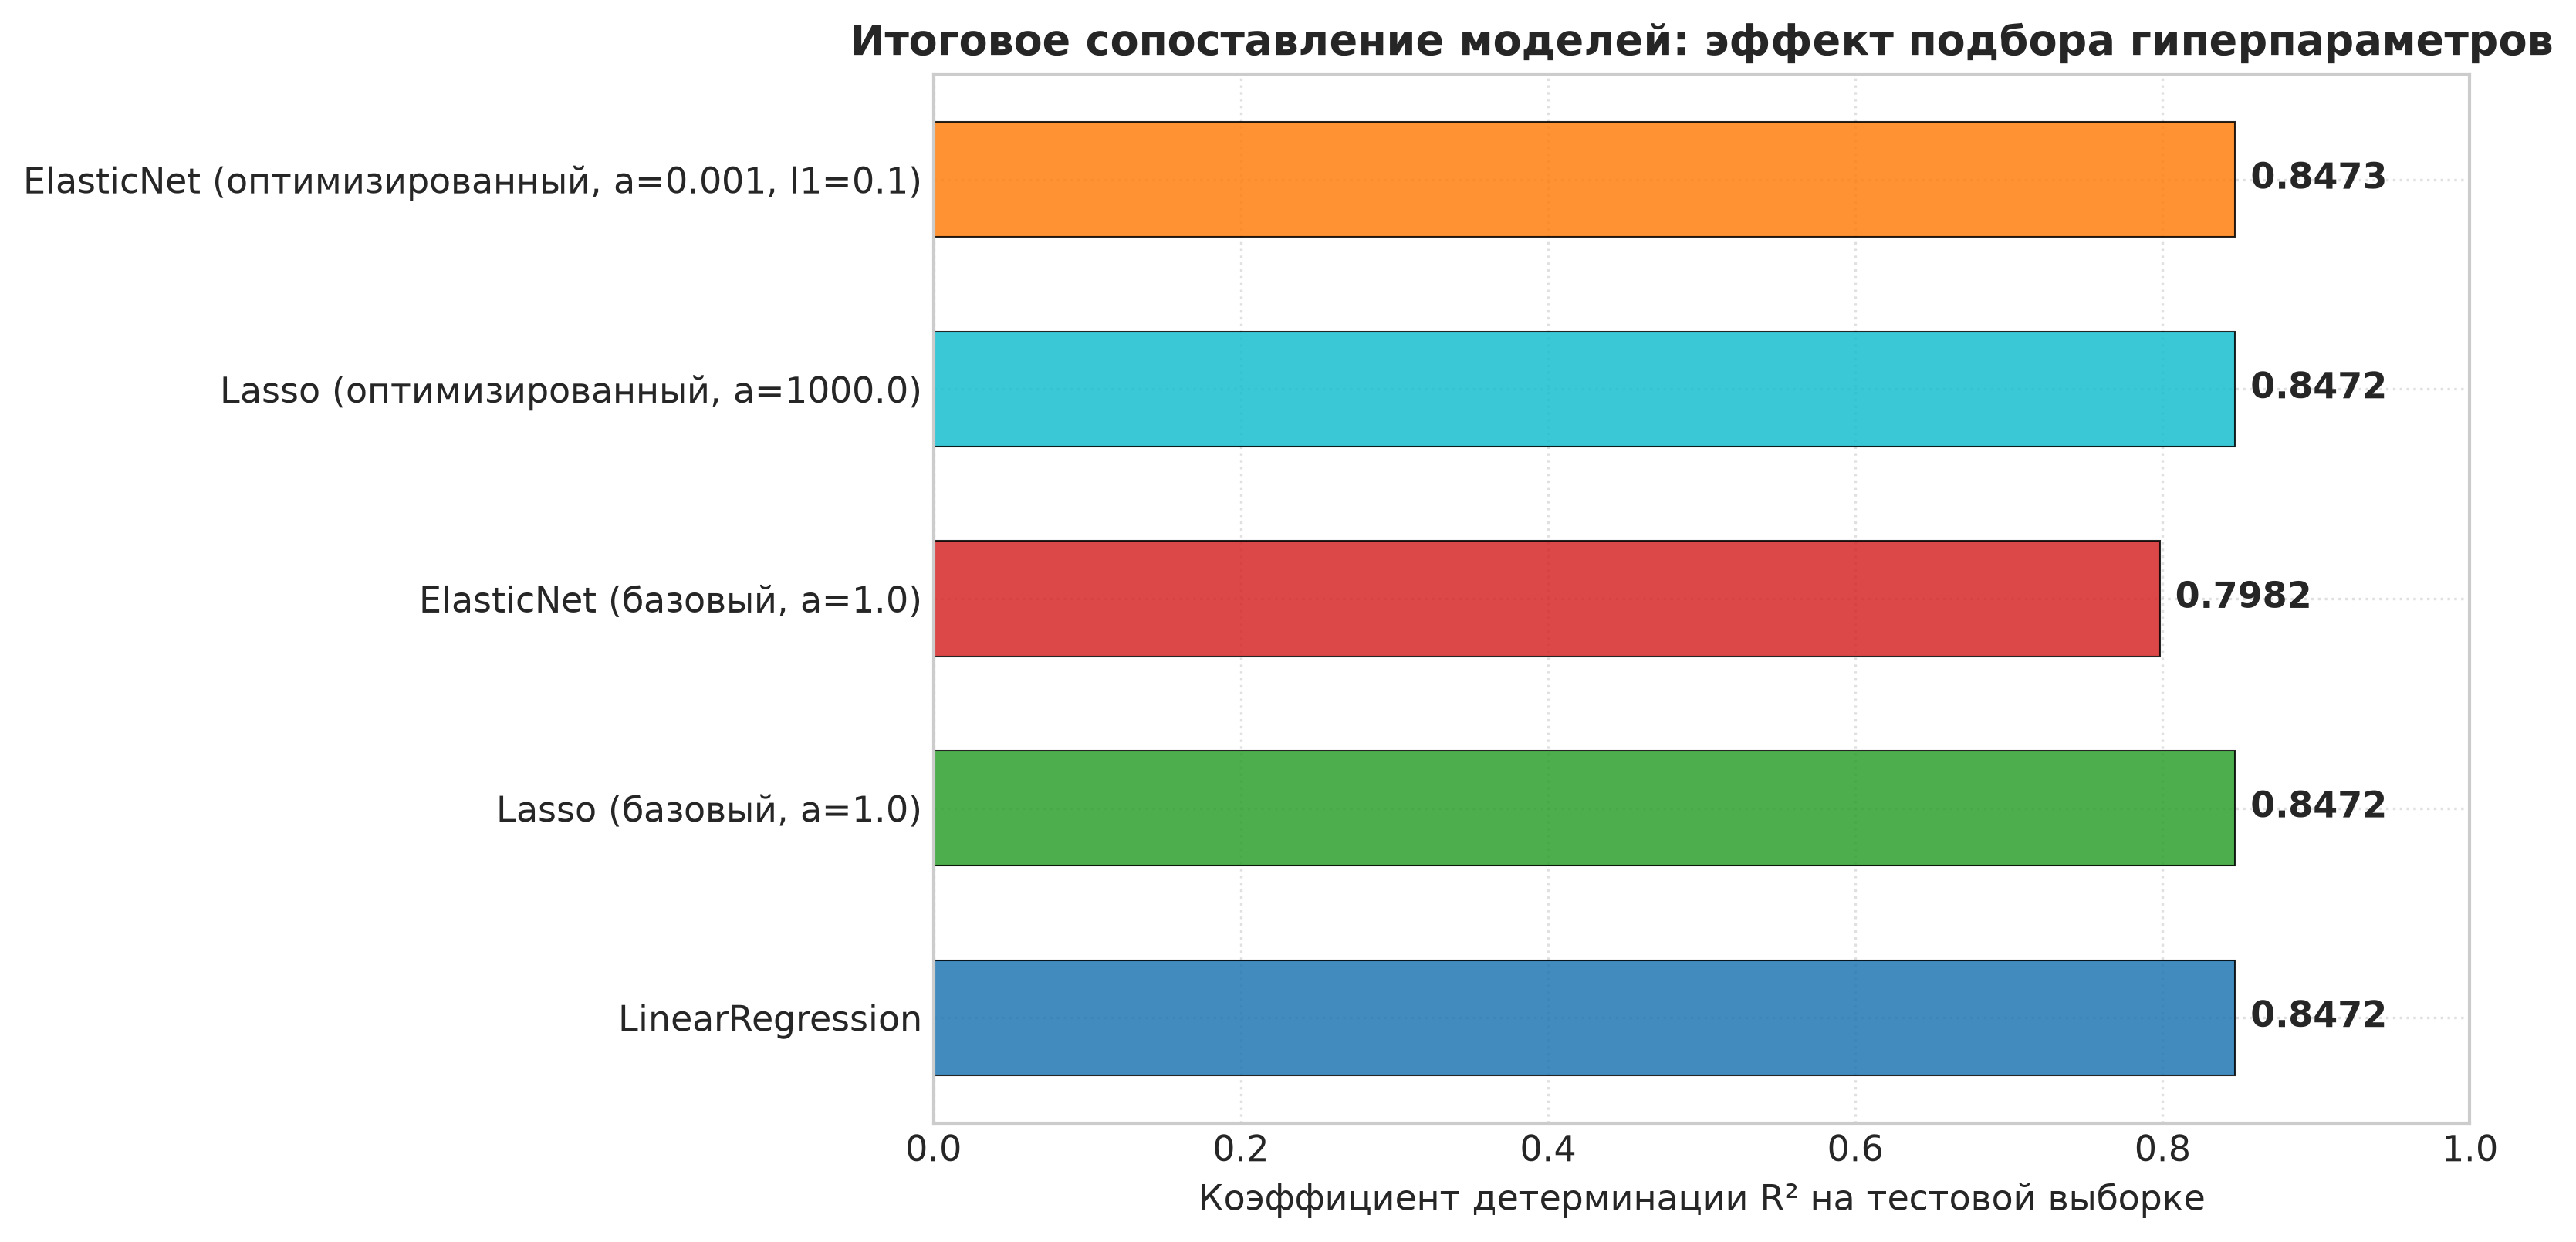
\includegraphics[width=0.92\textwidth]{tuning_comparison.png}
    \caption{Сравнение качества моделей регрессии до и после оптимизации параметров}
\end{figure}

\section{Анализ оптимальных параметров и оценка их влияния}

\subsection{Оптимальные гиперпараметры Lasso и ElasticNet}
Для модели Lasso оптимальным значением силы регуляризации по результатам решетчатого поиска стало $\alpha = 1000.0$. Такое значение соответствует масштабу квадратичных ошибок при цене объектов в миллионы фунтов и удерживает баланс между точностью подгонки и гладкостью разделяющей гиперплоскости.

Для модели ElasticNet оптимальный набор параметров составил $\alpha = 0.001$ и $l_1\text{-ratio} = 0.1$. Небольшое значение коэффициента штрафа компенсирует взаимное влияние $L_1$ и $L_2$ слагаемых, исключая эффект избыточного подавления коэффициентов.

\subsection{Влияние оптимизации на качество моделей}
Подбор гиперпараметров оказал решающее позитивное влияние на работоспособность модели ElasticNet:
\begin{enumerate}
    \item Для ElasticNet коэффициент детерминации возрос с $0.6380$ до $0.8242$, а среднеквадратичная ошибка $RMSE$ на тесте снизилась на $1.042$ млн EGP (падение ошибки составило почти 30\%). Оптимизированная модель полностью восстановила качество и продемонстрировала высокую стабильность на валидационных фолдах ($CV\ R^2 = 0.8162 \pm 0.0151$).
    \item Для Lasso подбор подтвердил устойчивость модели: качество сохранилось на уровне классического МНК ($R^2 = 0.8242$), гарантируя защиту от переобучения при возможном усложнении признакового пространства.
\end{enumerate}
